%%%%%%%%%%%%%%%%%%%%%%%%%%%%%%%%%%%%%%%%%%%%%%%%%%%%%%%%%%%%%%%%%%%
%%% Documento LaTeX 																						%%%
%%%%%%%%%%%%%%%%%%%%%%%%%%%%%%%%%%%%%%%%%%%%%%%%%%%%%%%%%%%%%%%%%%%
% Título:		Introducción
% Autor:  	Ignacio Moreno Doblas
% Fecha:  	2014-02-01, actualizado 2019-11-11
% Versión:	0.5.0
%%%%%%%%%%%%%%%%%%%%%%%%%%%%%%%%%%%%%%%%%%%%%%%%%%%%%%%%%%%%%%%%%%%
% !TEX root = A0.MiTFG.tex

\chapterbegin{Introducción y visión general}
\minitoc

%\begin{sinopsis}
%\label{sec:intro:sinop}
%
%Éste es el capítulo de introducción, donde se explica todo lo que un lector externo necesita para entender el resto de la documentación. El objetivo explica lo que persigue el proyecto, su finalidad.	El \miindex{estado del arte} explica la situación actual del entorno en el que este proyecto\footnote{En adelante, se utiliza la palabra \tit{proyecto} como sinónimo de TFG/TFM, según se aplique (Nota del autor).} se desenvuelve.
%
%Las metodologías y directrices seguidas se centran en qué procedimientos se han utilizado durante el desarrollo del proyecto. La estructura del documento describe los capítulos de los que se compone, incluyendo apéndices e información adicional. Por último, el ámbito de aplicación completa el entorno de utilización del proyecto.
%
%Aunque estos cinco apartados no son obligatorios, al menos es recomendable considerar estos conceptos en el capítulo de introducción como una guía básica. Tampoco es obligatorio usar el entorno \LaTeX\ \ttw{minitoc} para cada capítulo. En caso de no querer usarlo, tan sólo hay que comentar la línea \ttw{\textbackslash \miindex{minitoc}}. Igualmente, esta sección inicial de Sinopsis no es obligatoria, se puede suprimir si no se desea.
%
%Por extensión y en general, esta plantilla es una guía cuyo objetivo es facilitar la realización del proyecto, no un reglamento estricto ni rígido.
%\end{sinopsis}

\section{Estado del arte}

Como puede verse en la figura~\ref{fig:Muertes2016}, según la organización mundial de la salud (OMS) la principal causa de muertes en el mundo el año 2016 fuer una enfermedad isquémica del corazón y la segunda más relevante, los infartos. Además, cabe destacar que más del 75\% de las defunciones provocadas por enfermedades cardiovasculares se producen en países con bajos o medianos ingresos y que el 80\% de los infartos de miocardio y de los AVC (Accidente Vascular Cerebral) prematuros son prevenibles. Con estos datos parece razonable cualquier intento por desarrollar sistemas para mejorar la diagnosis y la prevención dichas enfermedades, de la forma más efectiva posible. Muchos de esto sistemas tienen como base de funcionamiento el registro no invasivo de la actividad eléctrica cardiaca, la denominada Electrocardiografía (ECG).. 

\begin{figure}[ht]
    \begin{minipage}[b]{\linewidth}
        \centering
        \subcaptionbox{Fallecimientos globales\label{subfig:Muertes2016}}
            {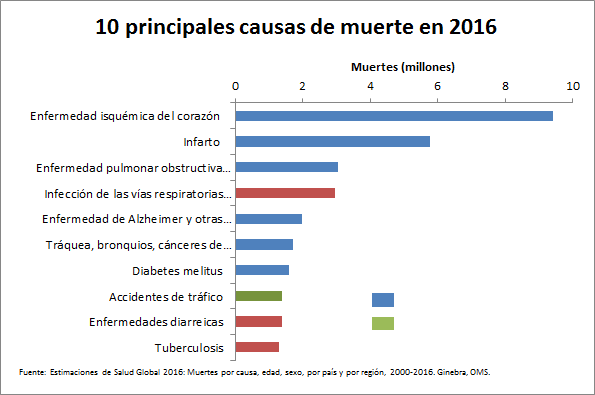
\includegraphics[width = .4\linewidth]{ figuras/Muertes2016.png}}
    \end{minipage}
            \begin{minipage}[b]{.5\linewidth}
        \centering
        \subcaptionbox{Fallecimientos en países con ingresos bajos-medios\label{subfig:Muertes2016Medio}}
            {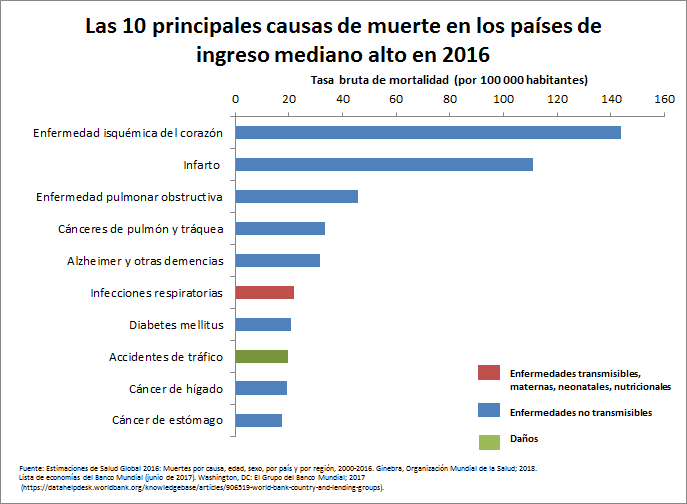
\includegraphics[width = .8\linewidth]{ figuras/Muertes2016MedioAlto.png}} 
    \end{minipage}
    \begin{minipage}[b]{.5\linewidth}
        \centering
        \subcaptionbox{Fallecimientos en países con ingresos altos\label{subfig:Muertes2016Alto}}
            {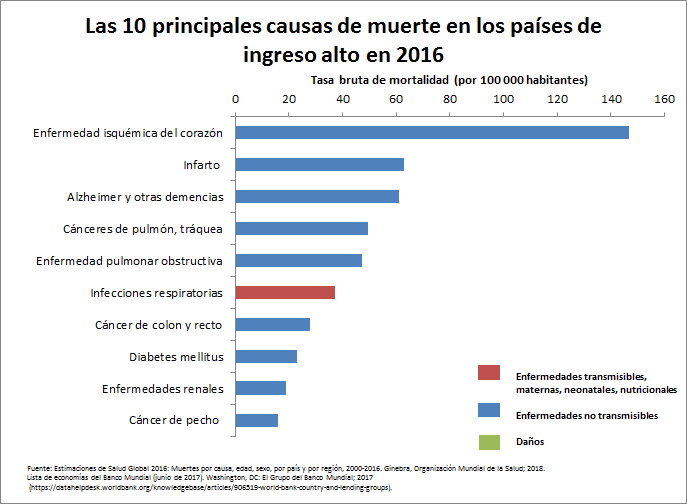
\includegraphics[width = .8\linewidth]{ figuras/Muertes2016Alto.png}}
        \end{minipage}
    \caption{Principales causas de muerte en 2016}
    \label{fig:Muertes2016}
\end{figure}

\subsection{Monitores portátiles de ECG}

Desde la década de los cuarenta se llevan investigando y mejorando dispositivos portátiles capaces de registrar las señales de ECG con el fin de obtener datos durante periodos extrahospitalarios. Concretamente el más antiguo de estos dispositivos es conocido como Holter, en honor a Norman J. Holter, quien desarrolló el primer prototipo en 1947, el cual pesaba alrededor de 38 Kg. No sería hasta el año 1962 cuando gracias a “Del Mar Engineering Laboratories” bajo el nombre de “Avionics Research Products Corporation” se consiguiera producir el primer dispositivo comercial, más ligero y capaz de almacenar el ECG de las últimas 24 horas. \cite{NormanHolter}

Desde sus inicios hasta hoy, el paradigma del registro de ECG portátil ha cambiado significativamente, gracias al desarrollo de la técnica, así como el uso de los monitores portátiles en la diagnosis y tratamiento de enfermedades cardiovasculares. En la actualidad hay dos tipos de dispositivos ampliamente utilizados, los ya mencionados monitores Holters y los monitores de eventos cardíacos. La principal diferencia entre ambos es la forma de almacenar los datos. Mientras que los holters registran los datos constantemente desde que el dispositivo es colocado por el médico hasta la consulta de vuelta, los monitores de eventos cardíacos son activados por los pacientes cuando padecen algún síntoma cardiovascular.

Teóricamente los monitores de eventos cardíacos son menos eficientes a la hora de la diagnosis de enfermedades que los Holters debido a que pierden los datos referentes a eventos que sean asintomáticos o que el paciente no percibe. Sin embargo encuentran su espacio en el mercado ya que típicamente son más pequeños y cómodos de usar que los Holters.

No obstante esto podría cambiar gracias al desarrollo de un nuevo tipo de monitores de eventos cardíacos, los supervisores de eventos cardíacos autodisparados. La teoría detrás de estos dispositivos es sencilla, si se puede analizar en tiempo real la señal ECG adquirida, entonces se puede detectar, en tiempo real y sin la intervención del paciente, el evento cardiaco anómalo. Y solo tras la detección, almacenar, e incluso trasmitir, el fragmento del ECG del paciente en el que se ha detectado el evento. Evitando así el enorme gasto de batería que conlleva la transmisión constante del registro y gozando de todas la ventajas de los supervisores cardíacos sin su mayor contra. La práctica, por otro lado, no es tan sencilla como se expondrá después.

La base del funcionamiento de un supervisor de eventos cardíaco autodisparados es la detección automática de los latidos presentes en la señal ECG.(TODO: Satija Reference) Localizados estos latidos, el supervisor debe extraer diversas características de ellos que permitan clasificarlos como anormales. La ocurrencia de estas anormalidades constituyen los eventos susceptibles de ser guardados o transmitidos.  Antes de continuar hablando de este tipo de monitores cardíacos es necesario comprender moderadamente los diferentes elementos de una señal ECG y qué datos médicos de interés se pueden obtener de ellos. 

\subsection{La señal ECG}

Como se puede ver en la figura~\ref{fig:ECGelements}, en la señal ECG correspondiente a un latido cardiaco, pueden apreciarse cinco elementos principales: la onda P, que representa la despolarización auricular, esto es, el latido de la aurícula; el complejo QRS, fruto de la despolarización ventricular, esto es, la contracción del ventrículo, y la onda T, que representa la repolarización ventricular, esto es, la relajación del ventrículo. Así, las ondas en sí mismas dan una idea de la actividad mecánica del corazón, y también se puede extraer mucha información de los intervalos entre las ondas, ya que reflejan las duraciones de los procesos biológicos del corazón.

%\begin{wrapfigure}{l}{0.5\linewidth}
\begin{figure}[ht]  
    \centering
        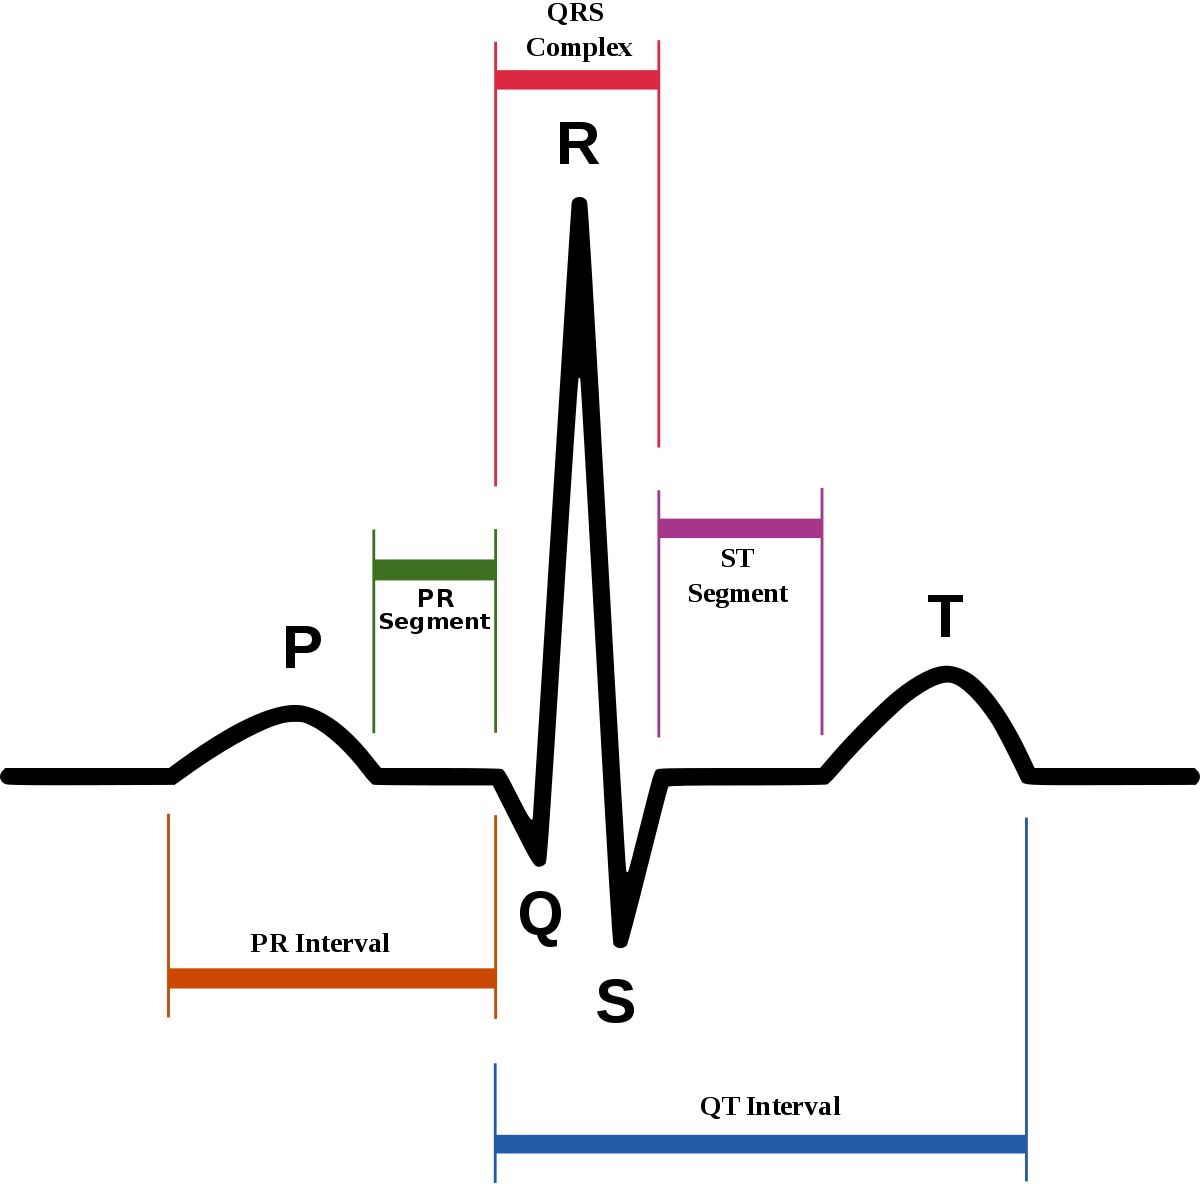
\includegraphics[width =0.4\linewidth]{figuras/ECGelementsDetailed.png}
    \caption{Elementos fundamentales ECG}
    \label{fig:ECGelements}
\end{figure}

En función de las posiciones donde se coloquen los electrodos a la hora de tomar las muestras, las señales se registrarán con una forma u otra. Estas posiciones se conocen como una derivaciones. En el ECG clásico estas derivaciones están estandarizadas en lo que se conoce como Sistema de doce derivaciones: un conjunto de seis derivaciones tomadas en las extremidades y otras seis, denominadas precordiales, que se sitúan en distintos puntos del torax. Las de las extremidades registran los potenciales que se transmiten al plano frontal y las precordiales recogen los potenciales del plano horizontal como puede verse en la figura \ref{fig:ECGelements}. \cite{Harrison}

Podría decirse que cada derivación hace las veces de un observador en un punto diferente, por lo que la señal resultante, que procede de diferencias potenciales con dirección y sentido, variará de polarización en según qué derivación, como puede “variar” el sentido de rotación de disco en función de si es observado desde arriba o desde abajo. La figura (TODO:Insertar referencia  1.2 ) en concreto corresponde a un ECG de un sujeto sano tomado en la derivación II.

\begin{figure}[ht]
	\centering
		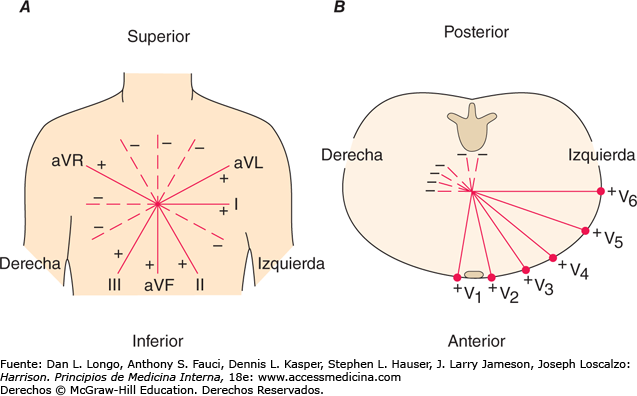
\includegraphics[width=0.9\linewidth]{figuras/derivations.png}
	\caption{Ilustración derivaciones ECG}
	\label{fig:derivaciones}
\end{figure} 

Desde que Willem Einthoven inventara el primer electrocardiograma hasta hoy la técnica ha mejorado enormemente y la precisión en las medidas hace posible observar fenómenos muy sutiles con un método de pruebas muy poco invasivo. La cantidad de patologías que pueden diagnosticarse realizando un electrocardiograma en el momento apropiado es enorme. \cite{PatologiasECG} Por ejemplificar esto, diremos que tan solo mediante la morfología de la onda P se pueden diagnosticar más de 15 patologías diferentes, por ejemplo, una fibrilación auricular cuando se hay una ausencia total de la onda o varios tipos de taquicardia, cuando se observan ausencias parciales. También se puede detectar un crecimiento auricular anormal si se observa que la onda es bifásica. Y un largo etcétera de patologías.

En muchas ocasiones la detección de estas patologías requiere como paso previo la detección del propio latido cardíaco. Una vez detectado se pueden realizar procesados complicados basados en la morfología de la onda u otros más sencillos como el cálculo de la tasa cardíaca, que pueden aportar mucha información.

\subsection{Detectores de QRS: cálculo de la tasa cardíaca basada en ECG}

Una vez reconocidos los latidos cardíacos se puede medir la diferencia de tiempo entre dos latidos, esto se conoce como intervalo RR (Ver figura~\ref{fig:RRInterval})  de donde se obtiene la frecuencia cardíaca instantánea, parámetro típico que es empleado para activar numerosos supervisores de eventos cardíacos autodisparados. Este proyecto se centra en este parámetro y, en particular, en los algoritmos de detección de latidos que posibilitan su obtención.  

\begin{figure}[ht]
	\centering
		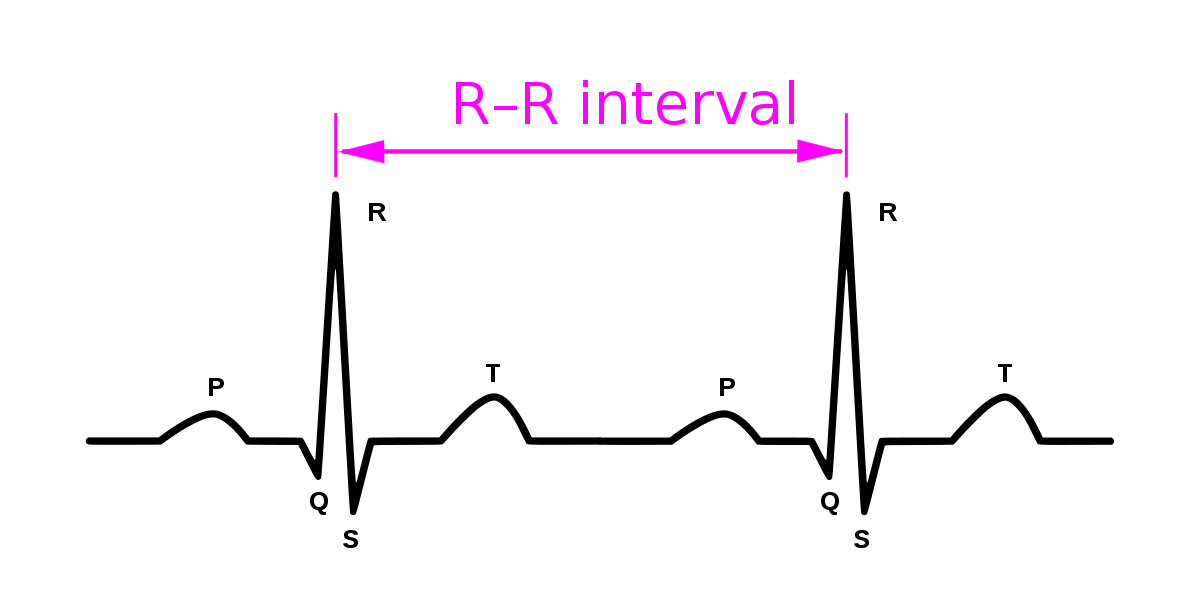
\includegraphics[width=0.6\linewidth]{figuras/RRInterval.png}
	\caption{Representación intervalo R-R}
	\label{fig:RRInterval}
\end{figure} 

En la literatura actual existen numerosos algoritmos muy testeados y eficaces a la hora de detectar el complejo QRS y ,en base a esa detección, calcular la tasa cardíaca. Tradicionalmente se ha desarrollado para ser ejecutados sobre unos datos extraídos previamente y almacenados en memoria. Pero esto no sirve para ser aplicados en tiempo real por diseño, así que en los últimos años se ha estado invirtiendo mucho esfuerzo en desarrollar algoritmos de tiempo real. Siendo el más conocido y uno de los más antiguos el de “Pan Tompkins” basado en el análisis de la pendiente, la intensidad y la duración de los complejos QRS.\cite{PanTompkins} A día de hoy se pueden encontrar numerosos estudios sobre nuevas metodologías para llevar a cabo esta tarea como algoritmos especializados en muestras con mucho ruido\cite{RsSlope} o métodos con diferentes aproximaciones como máquinas de estado finitas\cite{FSM} o empleando coeficientes de wavelet.\cite{Wavelet}

Sin embargo no resulta sencillo encontrar la forma de testar dichos métodos en entornos reales. Para realizar las pruebas pertinentes se hace uso de bases de datos estandarizadas como la MIT-BIH (TODO: Poner esto good con referencia y toh.), evaluando principalmente la tasa de falsos positivos y negativos. (TODO: Referencia Pootja 2017) Un ejemplo de algoritmo para determinar la fiabilidad de un algoritmo se puede encontrar en la norma para marcado CE de los Holter de ECG (TODO: referencia- AENOR, te la mando por correo)

Por otro lado, la tendencia actual es emplear dispositivos cada vez de menor consumo que suelen ir acompañados de menores recursos y baterías más pequeñas. Por ello cada vez se requieren métodos de detección con menor complejidad computacional pero con una robustez suficiente para ser caracterizados como fiables. Minimizando así las transmisiones de datos a lo estrictamente necesario, ahorrando batería para poder tomar medidas durante un periodo más largo. En este contexto resulta complejo evaluar cuando un algoritmo es suficientemente válido o no debido únicamente a su fiabilidad de detección, influyen también parámetros como el consumo de batería en ejecución, la necesidad de memora y la portabilidad de este a lenguajes de bajo nivel.

\subsection{Breves conclusiones}

Como se ha mencionado anteriormente las patologías cardíacas son una de las mayores causas de mortalidad en todo el mundo, por ende los supervisores de eventos cardiacos autodisparados podrían tener un efecto directo en la detección y seguimiento de estas patologías. La base principal de estos supervisores radica en la correcta detección de los complejos QRS, no solo de una forma fiable y en tiempo real, sino también con un consumo mínimo de recursos los recursos hardware del sistema.

\section{Objetivo}
%\label{sec:intro:obj}
%En esta sección, se describe el \miindex{objetivo del proyecto}, es decir, qué pretende, a qué aspira, cuál es su meta. Es importante comprender esta sección, porque de otro modo, no se entiende el resto de la documentación.
El objetivo de este proyecto es el diseño y la implementación de un entorno de pruebas genérico para testear diferente algoritmos de medida de tasa cardíaca instantánea basados en ECG en un entorno portátil de tiempo real con recursos limitados. Este entorno de pruebas será validado con un ejemplo concreto de algoritmo aplicado sobre señales ECG tomadas de la MIT-BIH.

Como objetivos personales de este proyecto se propusieron la profundización en los conocimientos sobre el procesado de datos, concretamente los datos de electrocardiogramas. Además se propuso emplear dicho proyecto para investigar y aprender a realizar documentación con \LaTeX
%\section{Metodología y directrices seguidas}


\section{Estructura del documento}
TODO: En esta sección, se explican los posteriores capítulos u otra información adicional que el proyecto contenga.

\chapterend
